\documentclass[12pt]{article} % use larger type; default would be 10pt

\usepackage{tikz}
\usepackage{pgfplots}
\usetikzlibrary{calc}
\usetikzlibrary{arrows.meta}
\usetikzlibrary{patterns}
        \newcommand\degree[0]{^{\circ}}
\usetikzlibrary{shapes.misc}

\title{Play with TikZ}
\author{Just Us}
%\date{} % Activate to display a given date or no date (if empty),
         % otherwise the current date is printed 

\begin{document}
\maketitle

\section{Chap 5 Equations and Identities}

\subsection{5.2 Solving Equations}

exam5-2-2 cubic $y=x^3-2x^2-5x$
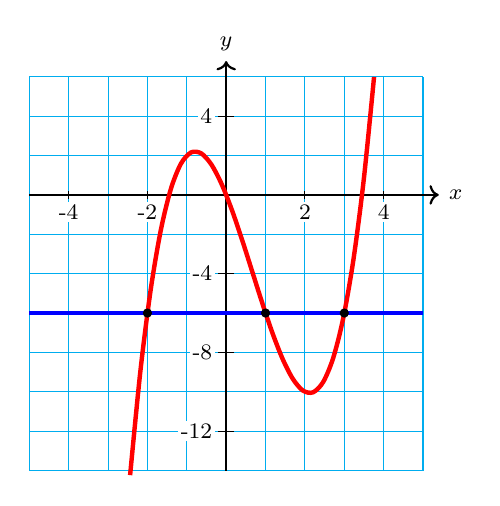
\begin{tikzpicture} [xscale=.5, yscale=.5]
\draw[cyan, ] (-5,-7) grid (5,3);
\draw[black, thick, ->] (-5,0) -- (5.4, 0) node[right]{\footnotesize$x$};
\draw[black, thick, ->] (0, -7) -- (0,3.4) node[above]{\footnotesize$y$};

\foreach \x in {-4, -2, 2, 4}
 \draw[black] (\x,0.1)--++(0,-0.2) node[below, fill=white, yshift=-1, inner sep = 1pt] {\footnotesize \x};
\foreach \y [evaluate=\y as \yi using int(2*\y)] in {-6, -4, -2, 2}
 \draw[black] (0.2,\y)--++(-0.4,0) node[left, fill=white, xshift=-1, inner sep = 1pt] {\footnotesize\yi};

\draw[domain=-2.44:3.756,smooth,variable=\x,red,ultra thick] plot ({\x},{(\x^3 -2*(\x)^2-5*\x)/2});
\draw[blue,very thick] (-5,-3)--++(10,0);

\filldraw[black] (-2,-3) circle (2.9pt);
\filldraw[black] (1,-3) circle (2.9pt);
\filldraw[black] (3,-3) circle (2.9pt);

\end{tikzpicture}
\newline



exer5-2-2ans
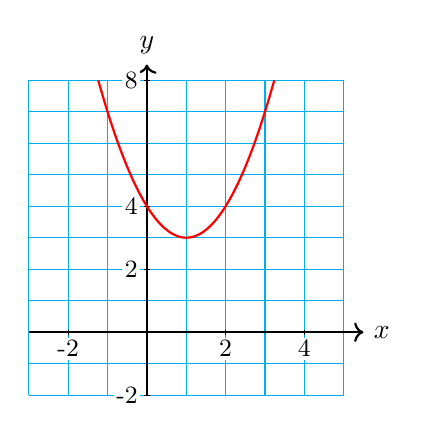
\begin{tikzpicture} [xscale=.5, yscale=.4]

\draw[cyan] (-3,-2) grid (5,8);
\draw[black, thick, ->] (-3,0)--(5.5,0) node[right]{$x$};
\draw[black, thick, ->] (0,-2)--(0,8.5) node[above]{$y$};
\foreach \x in {-2, 2, 4} 
 \draw[black] (\x,.08)--++(0,-.16) node[below, yshift=-1, fill=white, inner sep=1pt] {\small \x};
\foreach \y in {-2, 2, 4, 8} 
 \draw[black] (.08, \y)--++(-.16,0) node[left, xshift=-1, fill=white, inner sep=1pt] {\small \y};

\draw[domain=-1.235:3.236,smooth,variable=\x,red, thick] plot ({\x},{(\x)^2 - 2*\x + 4 });

\end{tikzpicture}
\newline



fig-5-2-ferris

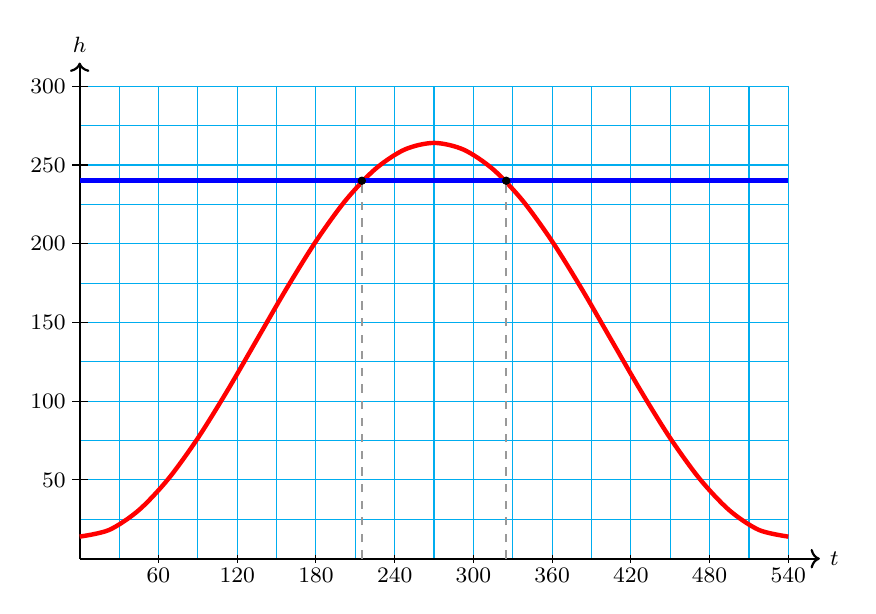
\begin{tikzpicture} [xscale=.5, yscale=.5]
\draw[cyan, ] (0,0) grid (18,12);
\draw[black, thick, ->] (0,0) -- (18.8, 0) node[right]{\footnotesize$t$};
\draw[black, thick, ->] (0, 0) -- (0,12.6) node[above]{\footnotesize$h$};

\foreach \x [evaluate=\x as \xi using int(30*\x)] in {2, 4, ..., 18}
 \draw[black] (\x,0.1)--++(0,-0.2) node[below, fill=white, yshift=-1, inner sep = 1pt] {\footnotesize \xi};
\foreach \y [evaluate=\y as \yi using int(25*\y)] in {2, 4, ..., 12}
 \draw[black] (0.2,\y)--++(-0.4,0) node[left, fill=white, xshift=-1, inner sep = 1pt] {\footnotesize\yi};

\draw[domain=0:18,smooth,variable=\x,red,ultra thick] plot ({\x},{ 139/25 - 5* cos(30 * 2 * \x /3 });
\draw[blue,ultra thick] (0,240/25)--++(18,0);

\draw[gray!80!white, thick, dashed] (215/30, 0) -- ++(0,240/25);
\draw[gray!80!white, thick, dashed] (325/30, 0) -- ++(0,240/25);

\filldraw[black] (215/30, 240/25) circle (2.6pt);
\filldraw[black] (325/30, 240/25) circle (2.6pt);

\end{tikzpicture}
\newline


fig-5-2-eqn
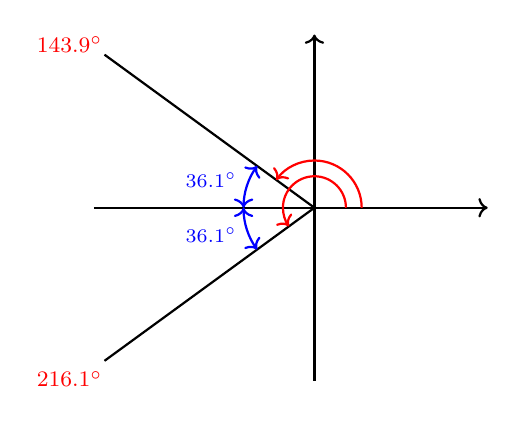
\begin{tikzpicture}

\draw[black,thick,->] (-2.8,0)--++(5,0);
\draw[black,thick,->] (0,-2.2)--++(0,4.4);

\coordinate (O) at (0,0);
\coordinate (A) at (143.9:3.3);
\coordinate (B) at (216.1:3.3);

\draw[black,thick] (O)--(A) node[anchor=south east, xshift=3, yshift=-3]{\color{red}\footnotesize$143.9\degree$};
\draw[black,thick] (O)--(B) node[anchor=north east, xshift=3]{\color{red}\footnotesize$216.1\degree$};

\draw[blue, thick, <->] (180:.9) arc (180:143.9:0.9) node[left, midway, yshift=2] {\scriptsize$36.1\degree$};
\draw[blue, thick, <->] (180:.9) arc (180:216.1:0.9) node[left, midway, yshift=-2] {\scriptsize$36.1\degree$};
\draw[red, thick, ->] (0:.4) arc (0:216.1:0.4);
\draw[red, thick, ->] (0:.6) arc (0:143.9:0.6);

\end{tikzpicture}
\newline


exam5-2-3
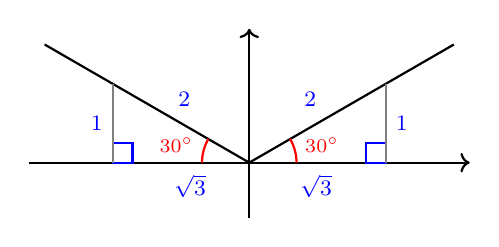
\begin{tikzpicture}

\draw[black,thick,->] (-2.8,0)--++(5.6,0);
\draw[black,thick,->] (0,-.7)--++(0,2.4);

\coordinate (O) at (0,0);
\coordinate (A) at (30:3);
\coordinate (B) at (150:3);
\coordinate (C) at ($ sqrt(3)*(1,0)$);
\coordinate (D) at ($ -sqrt(3)*(1,0)$);

\draw[black,thick] (B)--(O)--(A) ;

\draw[red, thick] (180:.6) arc (180:150:0.6) node[left, midway, yshift=2] {\scriptsize$30\degree$};
\draw[red, thick] (0:.6) arc (0:30:0.6) node[right, midway, yshift=2] {\scriptsize$30\degree$};
\draw[blue,thick] (C) rectangle ++(-.25,.25);
\draw[blue,thick] (D) rectangle ++(.25,.25);
\draw[gray, thick] (C)--++(0,1) node[right, midway]{\footnotesize\color{blue}1};
\draw[gray, thick] (D)--++(0,1) node[left, midway]{\footnotesize\color{blue}1};

\node[text width=.3cm] at (.8,-.3)    {\color{blue}\footnotesize$\sqrt{3}$};
\node[text width=.3cm] at (-.8,-.3)    {\color{blue}\footnotesize$\sqrt{3}$};
\node[text width=.2cm] at (-.8,.8)    {\color{blue}\footnotesize 2};
\node[text width=.2cm] at (.8,.8)    {\color{blue}\footnotesize 2};

\end{tikzpicture}
\newline


fig-5-2-infsoln

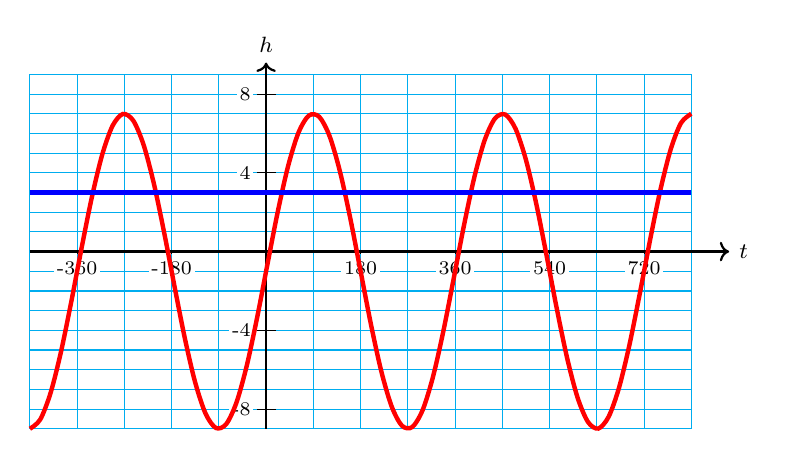
\begin{tikzpicture} [xscale=.6, yscale=.25]
\draw[cyan, ] (-5,-9) grid (9,9);
\draw[black, thick, ->] (-5,0) -- (9.8, 0) node[right]{\footnotesize$t$};
\draw[black, thick, ->] (0, -9) -- (0,9.6) node[above]{\footnotesize$h$};

\foreach \x [evaluate=\x as \xi using int(90*\x)] in {-4,-2, 2,4,6,8}
 \draw[black] (\x,0.1)--++(0,-0.2) node[below, fill=white, yshift=-2, inner sep = 1pt] {\scriptsize \xi};
\foreach \y [evaluate=\y as \yi using int(1*\y)] in {-8, -4, 4, 8}
 \draw[black] (0.2,\y)--++(-0.4,0) node[left, fill=white, xshift=-1, inner sep = 1pt] {\scriptsize\yi};

\draw[samples=65,domain=-5:9,smooth,variable=\x,red,ultra thick] plot ({\x},{ -1 + 8* sin(90* \x  });
\draw[blue,ultra thick] (-5,3)--++(14,0);

\end{tikzpicture}
\newline


exam5-2-4
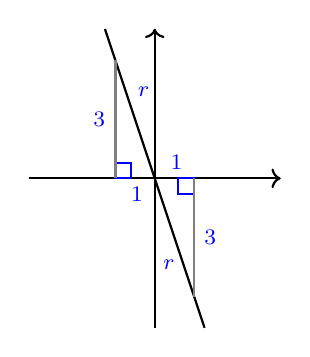
\begin{tikzpicture}

\draw[black,thick,->] (-1.6,0)--++(3.2,0);
\draw[black,thick,->] (0,-1.9)--++(0,3.8);

\coordinate (O) at (0,0);
\coordinate (A) at ({180-atan(3)}:2.);
\coordinate (B) at ({-atan(3)}:2.);

\draw[black,thick] (B)--(O)--(A) ;

\draw[blue,thick] (.5,0) rectangle ++(-.2,-.2);
\draw[blue,thick] (-.5,0) rectangle ++(.2,.2);
\draw[gray, thick] (.5,0)--++(0,-1.5) node[right, midway]{\footnotesize\color{blue} 3};
\draw[gray, thick] (-.5,0)--++(0,1.5) node[left, midway]{\footnotesize\color{blue} 3};

\node[text width=.1cm] at (.25,.2) {\color{blue}\footnotesize 1};
\node[text width=.1cm] at (-.25,-.2) {\color{blue}\footnotesize 1};
\node[text width=.1cm] at (-.16,1.1) {\color{blue}\footnotesize $r$};
\node[text width=.1cm] at (.16,-1.1){\color{blue}\footnotesize $r$};

\end{tikzpicture}
\newline


exam5-2-6 tangent graph
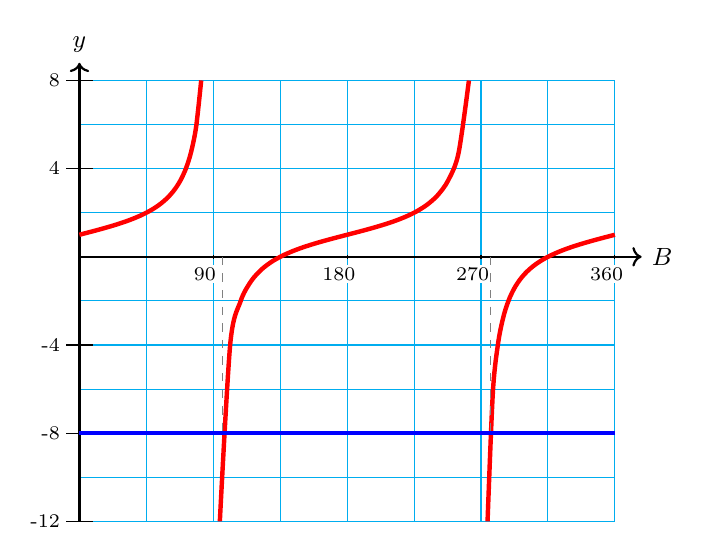
\begin{tikzpicture} [xscale=.85, yscale=.28]

\draw[cyan, ystep=2] (0,-12) grid (8,8);
\draw[black,thick,->] (0,0)--(8.4,0) node[right]{\small$B$};
\draw[black,thick,->] (0,-12)--(0,8.8) node[above]{\small$y$};

\foreach \x [evaluate=\x as \xi using int(45*\x)] in {2, 4, 6, 8}
 \draw[black] (\x,0.1)--++(0,-0.2) node[below, fill=white, xshift=-3, yshift=-2, inner sep = 1pt] {\scriptsize \xi};
\foreach \y [evaluate=\y as \yi using int(1*\y)] in {-12, -8, -4, 4, 8}
 \draw[black] (0.2,\y)--++(-0.4,0) node[left, fill=white, xshift=-1, inner sep = 1pt] {\scriptsize\yi};
 
\draw[domain={0:atan(7)/45},smooth,variable=\x,red,ultra thick] plot ({\x},{ 1+tan(45* \x)  });
\draw[domain={4-atan(13)/45:4+atan(7)/45},smooth,variable=\x,red,ultra thick] plot ({\x},{ 1+tan(45* \x)  });
\draw[domain={8-atan(13)/45:8},smooth,variable=\x,red,ultra thick] plot ({\x},{ 1+tan(45* \x)  });

\draw[blue,ultra thick] (0,-8)--(8,-8);
\coordinate (A) at ($ atan(-9)/45*(1,0)+(4,0) $);
\draw[gray, dashed] (A) --++(0,-8);
\coordinate (B) at ($ atan(-9)/45*(1,0)+(8,0) $);
\draw[gray, dashed] (B) --++(0,-8);

\end{tikzpicture}
\newline



exer5-2-6ans cosine graph
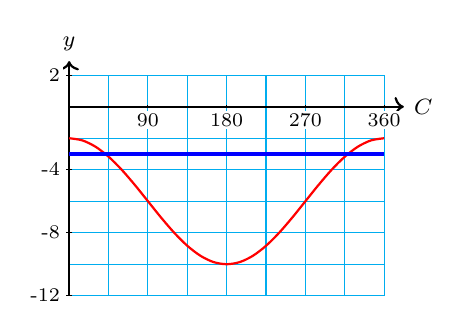
\begin{tikzpicture} [xscale=.5, yscale=.2]

\draw[cyan, ystep=2] (0,-12) grid (8,2);
\draw[black, thick, ->] (0,0)--(8.5,0) node[right]{\footnotesize$C$};
\draw[black, thick, ->] (0,-12)--(0,2.9) node[above]{\footnotesize$y$};
\foreach \x [evaluate=\x as \xi using int(45*\x)] in {2, 4, 6, 8} 
 \draw[black] (\x,.08)--++(0,-.16) node[below, yshift=-1, fill=white, inner sep=1pt] {\scriptsize \xi};
\foreach \y in {-12, -8, -4,2} 
 \draw[black] (.08, \y)--++(-.16,0) node[left, xshift=-1, fill=white, inner sep=1pt] {\scriptsize \y};

\draw[domain=0:8,smooth,variable=\x,red, thick] plot ({\x},{4*cos(45*\x) - 6 });
\draw[blue, very thick] (0,-3)--++(8,0);

\end{tikzpicture}
\newline


exam5-2-7
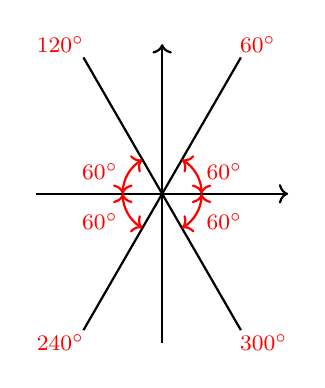
\begin{tikzpicture}

\draw[black,thick,->] (-1.6,0)--++(3.2,0);
\draw[black,thick,->] (0,-1.9)--++(0,3.8);

\coordinate (O) at (0,0);
\coordinate (A) at (60:2.);
\coordinate (B) at (120:2.);
\coordinate (C) at (240:2.);
\coordinate (D) at (300:2.);

\draw[black,thick] (O)--(A) node[above right, xshift=-4, yshift=-2]{\footnotesize \color{red}$60\degree$};
\draw[black,thick] (O)--(B) node[above left, xshift=4, yshift=-2]{\footnotesize \color{red}$120\degree$};
\draw[black,thick] (O)--(C) node[below left, xshift=4, yshift=2]{\footnotesize \color{red}$240\degree$};
\draw[black,thick] (O)--(D) node[below right, xshift=-4, yshift=2]{\footnotesize \color{red}$300\degree$};

\draw[red,thick, <->] (.5,0) arc (0:60:.5) node[right, midway, yshift=1] {\footnotesize $60\degree$};
\draw[red,thick, <->] (-.5,0) arc (180:120:.5) node[left, midway, yshift=1] {\footnotesize $60\degree$};
\draw[red,thick, <->] (-.5,0) arc (180:240:.5) node[left, midway, yshift=-3] {\footnotesize $60\degree$};
\draw[red,thick, <->] (.5,0) arc (0:-60:.5) node[right, midway, yshift=-3] {\footnotesize $60\degree$};

\end{tikzpicture}
\newline

fig-5-2-snell Snell's law

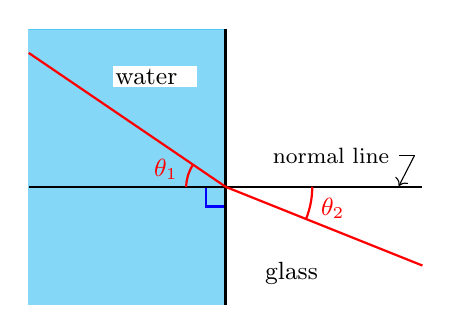
\begin{tikzpicture} 

\coordinate (O) at (0,0);
\coordinate (A) at (-2.5,-1.5);
\coordinate (B) at (-2.5,2);
\coordinate (C) at (0,2);
\coordinate (D) at (0,-1.5);
\coordinate (E) at (-2.5,1.7);
\coordinate (F) at (2.5,-1);


\draw[draw=cyan!80!white, fill=cyan!80!white, opacity=.6] (A)--(B)--(C)--(D);
\draw[blue, thick] (O) rectangle ++(-.25, -.25);
\draw[black, thick] (-2.5,0)--(2.5,0);
\draw[black, very thick] (0,-1.5)--(0,2);
\draw[red, thick] (E)--(O)--(F);
\draw[red, thick] (-.5,0) arc (180:{180-atan(1.7/2.5)}:.5) node[left, midway, yshift=2] {\small $\theta_1$};
\draw[red, thick] (1.1,0) arc (0:{-atan(1/2.5)}:1.1) node[right, midway, yshift=-2] {\small $\theta_2$};

\node [text width=1cm, fill=white, inner sep=1pt] at (-.9,1.4) {\small water};
\node [text width=1cm, fill=white, inner sep=1pt] at (1,-1.1) {\small glass};
\coordinate (N) at (2.4,.4);
\draw[black] (N)--++(-.2,0) node[left]{\footnotesize normal line};
\draw[black, ->] (N)--++(-.2,-.39)  ;
\end{tikzpicture}
\newline





\end{document}
